
\documentclass{article}
\usepackage{neurips_2023}
\usepackage[utf8]{inputenc}
\usepackage{geometry}
\usepackage{fancyhdr}
\usepackage{amsmath}
\usepackage{amssymb}
\usepackage{xspace}
\usepackage{bm}
\usepackage{xcolor}
\usepackage[colorlinks,linkcolor=blue]{hyperref}
\usepackage{graphicx}
\usepackage{url}
\usepackage{float}


\makeatletter
\DeclareRobustCommand\onedot{\futurelet\@let@token\@onedot}
\def\@onedot{\ifx\@let@token.\else.\null\fi\xspace}
\def\iid{\emph{i.i.d}\onedot} \def\IID{\emph{I.I.D}\onedot}
\def\eg{\emph{e.g}\onedot} \def\Eg{\emph{E.g}\onedot}
\def\ie{\emph{i.e}\onedot} \def\Ie{\emph{I.e}\onedot}
\def\cf{\emph{c.f}\onedot} \def\Cf{\emph{C.f}\onedot}
\def\etc{\emph{etc}\onedot} \def\vs{\emph{vs}\onedot}
\def\wrt{w.r.t\onedot} \def\dof{d.o.f\onedot}
\def\aka{\emph{a.k.a}\onedot}
\def\etal{\emph{et al}\onedot}
\makeatother

\newcommand{\important}[1]{{\color{blue}{\bf\sf #1}}}

\title{CPEN455 Final Project: PixelCNN++G}
\author{
  Guan Zheng Huang \\
  CPEN 455\\
  UBC\\
}


\begin{document}

\pagestyle{fancy}
\fancyhead{} 
\fancyhead[L]{\textbf{UBC CPEN455 2023 Winter Term 2}}
\fancyhead[R]{\textbf{Final Project: PixelCNN++G}}

\maketitle
\thispagestyle{fancy}

\begin{abstract}
    PixelCNN++G is a conditional generative model based on the PixelCNN++ architecture[2]. For this project, we aim to implement the PixelCNN++G model with an additional classification layer to transform it into an image classification model. The model will be trained on the CPEN450 dataset to classify images into one of four classes.
  \end{abstract}

\section{Model}

\subsection{PixelCNN++G Improvements}

    \subsubsection{Data Preprocessing:}
    \begin{itemize}
        \item PixelCNN is orientation-sensitive, which means it has difficulty recognizing the orientation of objects. To address this, we randomly flip the images horizontally during training to make the model invariant to the direction of the image. This technique is also equivalent to introducing double the amount of training data, which can help improve the model's generalization ability.
        \item Additionally, we rotate the images randomly form -10 to +10 degrees so that the model can learn object orientations with reduced impact from the image directionality.
        \item We introduced various new data augmentation techniques during the fine-tuning process, in hope to generate more data unfamiliar to the model, which is often desired for th fine-tuning process. This includes colour jittering and random cropping. Based on measure, fine-process with this technique increased accuracy by 2.00\% on validation dataset, 1.54\% on test dataset.
    \end{itemize}

    \subsubsection{Conditional Model:}
    \begin{itemize}
        \item The model is conditioned on the class label of the image, which is incorporated as an additional input. 
        \item Among the \texttt{gated\_resnet} function, we introduced two new weights layer, each of which is multiped with input label. The result is added to the resulting \texttt{a}, \texttt{b} parameters after the convolution operations. We used the same weights through all layers of the model. Pooling when necessary to match the dimensions of the input and output with the expectation that pixels would be influenced similarly by the weights, regardless of the layers. While such assumption maybe challenged by the existence of the skip connections, such technique still showed superior result to the approach of independent learning the weights at each layer.
     \end{itemize}

    \subsubsection{Classification Layer:}
    \begin{itemize}
        \item We employ the loss function as the classification layer. The idea is that by iterating over an image with all possible labels, the label that results in the lowest loss is chosen as the predicted label by the model. This method offers a straightforward and effective means of classification without the need for additional layers or parameters.
    \end{itemize}
% TODO: TEST pp, TEST base, classification layer, embedding, finetuning, 

\section{Experiments}
The model is trained on the CPEN450 dataset, 32x32 pixel images divided into four classes. With a batch size of 16 with 500 epochs, the additional conditional parameters are trained with xavier uniform initialization. The fid curve can be found on Figure \ref{fig:o-fid} and the BPD curve can be found on Figure \ref{fig:o-bpd}.
Sample images are shown in Figure \ref{fig:sample}.

\begin{figure}
    \centering
    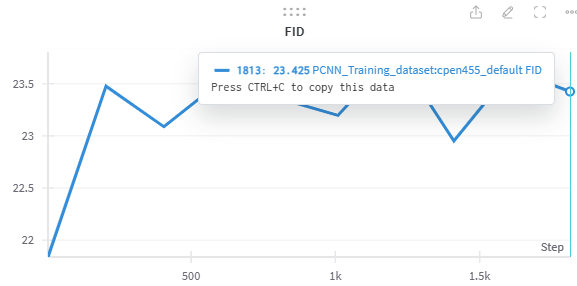
\includegraphics[width=0.5\textwidth]{report_data/o-fid.png}
    \caption{ FID curve for the main model.}
    \label{fig:o-fid}
  \end{figure}

  \begin{figure}
    \centering
    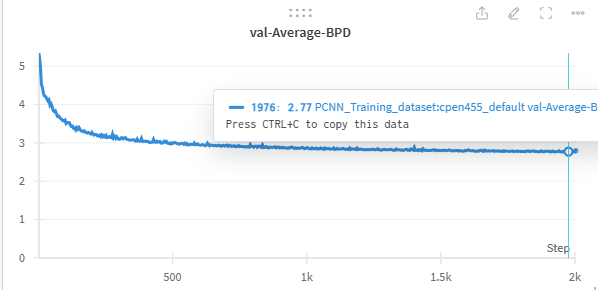
\includegraphics[width=0.5\textwidth]{report_data/o-bpd.png}
    \caption{ FID curve for the main model.}
    \label{fig:F-FID}
  \end{figure}

  \begin{figure}
    \centering
    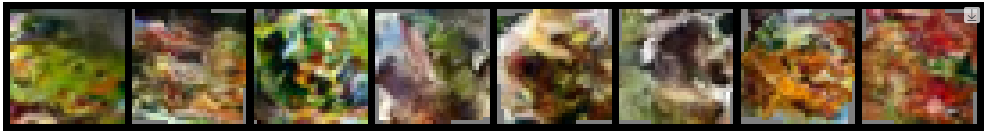
\includegraphics[width=0.9\textwidth]{report_data/o-1.png}
    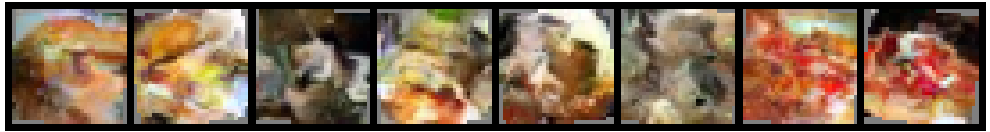
\includegraphics[width=0.9\textwidth]{report_data/o-2.png}
    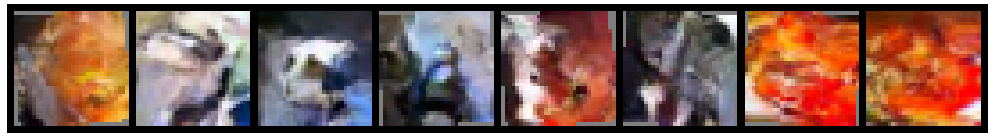
\includegraphics[width=0.9\textwidth]{report_data/o-3.png}
    \caption{ Sample images generated by the model. Counting from left column to right column, the first column is the class0, the second column is the class1, the third column is the class2, and the fourth column is the class3.}
    \label{fig:sample}
  \end{figure}

\subsection{major hyperparameter}
\begin{verbatim}
--batch_size 16 `
--nr_resnet 2 `
--nr_filters 160 `
--nr_logistic_mix 100 `
--lr_decay 0.99995 `
--max_epochs 500 `
--seed 4399
\end{verbatim}

\subsection{Training and setup}
The code consist of only packages listed under requirements.txt. The code is run on a single 2070 super max-Q mobile GPU. The training process took approximately 24 hours to complete. Cuda version is 12.4.131, the torch version is cuda121, python version is 3.10.13. 

\subsection{GPT-Use}
Sections of the code modified by GPT is labeled in line with comment. One can find the chat history with GPT in the supplementary materials section

\subsection{Results}
With the model trained, we achieved an accuracy of 44\% on the test set. The model is able to classify images into the correct class with reasonable accuracy.

\subsection{Alternative solutions attempted}

Several other solutions were attempted but did not show as promising results are discussed below. Unless explicitly stated, all structures are trained with hyperparameter [resnet = 1, filter = 40, logistical\_mix = 10] at 200 epochs without finetuning. Measured accuracy is taken among the highest of all checkpoints. For reference, the reduced parameter model demonstrated an accuracy of 65.1\% on the validation dataset at epoch 200 with 37.6 FID, and 71.0 \% at epoch 350 (optimal amongst 500 epoch). The FID score is 28.7 at epoch 350.

\begin{itemize}
    \item Specialized preprocessing techniques, such as image segmentation and swapping, noise and data masking did not prove to aid the training nor finetuning of the model. Such observation may largely be due to the limited training data and pixelCNN's nature of per pixel generation. Validation accuracy reduced from 65.1\% to 63.3\%. 
    \item To embed the label information in the model, attempts were made to embed label information directly into the input or output of the model, which failed to show significant improvement in classification accuracy. The same attempt was made in combination with the proposed weight application technique in resnet blocks, which also failed to show improvement in classification accuracy. Validation accuracy of 53.2\% is shown with 500 epochs.
    \item Attempts to utilizing a Polyak Averaged Model to be embedded and concatenated with the input at the ResNet block level have also been studied. While this approach showed promising results in terms of the Fréchet Inception Distance (FID), it did not significantly improve classification accuracy. Validation accuracy of 67.2\% is shown with 450 epochs.
    \item A major model restructure to incorporate a label channel also showed limited success. This approach failed to improve classification accuracy beyond random guessing. Inspecting the generated images, it is observed that the model is unable to generate images that resemble the input images. This may suggest a structural or programming failure which failed to properly handle the label layer. Example images generated by this model are shown in Figure \ref{fig:F-lc-sample}. The best validation accuracy is 25.2\% among 400 epochs, with 28.7 FID for that checkpoint.
    
    \item Additional attempt to modify the PCNN++G structure by updating the resnet structure by removing final addition with input matrix, instead purely depending on convolution layers to transform the input have been made. Although this method produced reasonable FID score of 25.5 at epoch 200 with, it marley achieved a classification accuracy of 49.2\%. 
    \item In this solution, we modified PixelCNNLayer\_up\/down and Resnet to introduces a new set of weights at every layer of both the upward and downward paths (6 layers in total, 8 at each resnet, each coming into effect based on the label). These weights are multiplied by the class label embedding before being applied in the convolution layers. This operation is by pixel, meaning that theoretically, as unique weight can be learned about each pixel at each layer. It will establish a stronger correlation between specific components of the image and its class at every layer to address the difficulty of model capturing label information. This strategy, in combination with the proposed tanh normalization technique introduced in [1] also showed promising results of 68.4\% validation accuracy at epoch 225. However, this approach showed signs of ovefitting, dispite the fact that there is increasing in parameter count. The BPD curve is shown in Figure \ref{fid:F-BPD}. 
    \item Reflecting on top of the above approach, we removed the dependency of the model on specific labels, instead introducing a single wight matrix that is multiplied with the labels, normalized and added to the output. Indeed, we no longer observe the overfitting issue, and the model achieved a validation accuracy of 71.8\% at epoch 500. The FID score is sub 20 at times. The only reason this model is not chosen as the final model is due to the fact that the model is not able to generalize well to the test dataset at high parameter count. The best performing checkpoint for [resnet = 1, filter = 128, logistical\_mix = 100] model achieved a test accuracy of XXX. The comparison between this model and the proposed model is shown in Figure \ref{fig:f_pp_cmp}
\end{itemize}

\begin{figure}
    \centering
    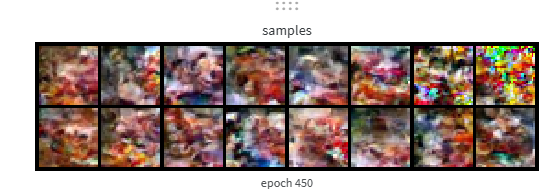
\includegraphics[width=0.5\textwidth]{report_data/f-lc-samples.png}
    \caption{ Sample images generated by the model with label as channel.}
    \label{fig:f-lc-samples}
\end{figure}

\begin{figure}
    \centering
    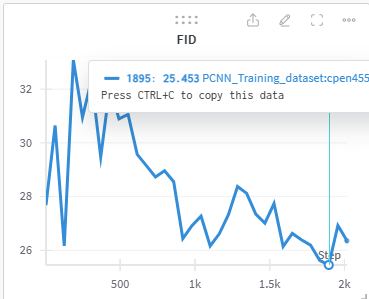
\includegraphics[width=0.5\textwidth]{report_data/f_1_fid.png}
    \caption{ FID curve for the model with different down-sampling weights for each class.}
    \label{fig:F-FID}
  \end{figure}

\begin{figure}
    \centering
    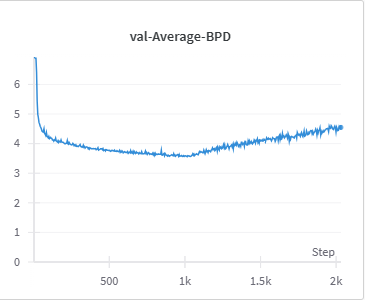
\includegraphics[width=0.5\textwidth]{report_data/f_2_BPD.png}
    \caption{BPD curve for the model with new set of weights at every layer.}
    \label{fig:F-BPD}
  \end{figure}
  \begin{figure}
    \centering
    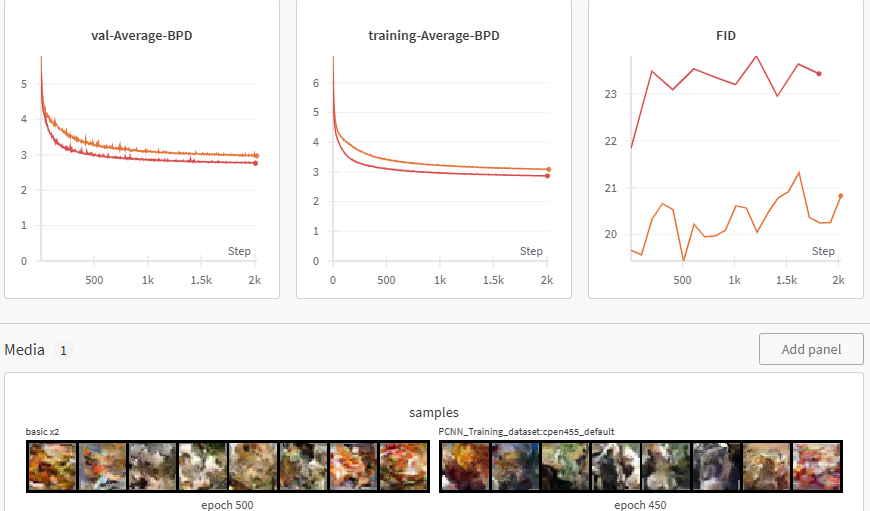
\includegraphics[width=0.5\textwidth]{report_data/f_pp_cmp.png}
    \caption{Comparison between the final model and the model with different down-sampling weights for each class.}
    \label{fig:F-BPD}
  \end{figure}

\section{Conclusion}

In conclusion, the modifications from the author, the PixelCNN++G model was able to achieve a classification accuracy of 36.8\% on the CPEN450 dataset, with a FID score of 32.73. The model and corresponding code is included as appendix to this report.


\section{Supplementary Material}

\begin{figure}[H]
    \centering
    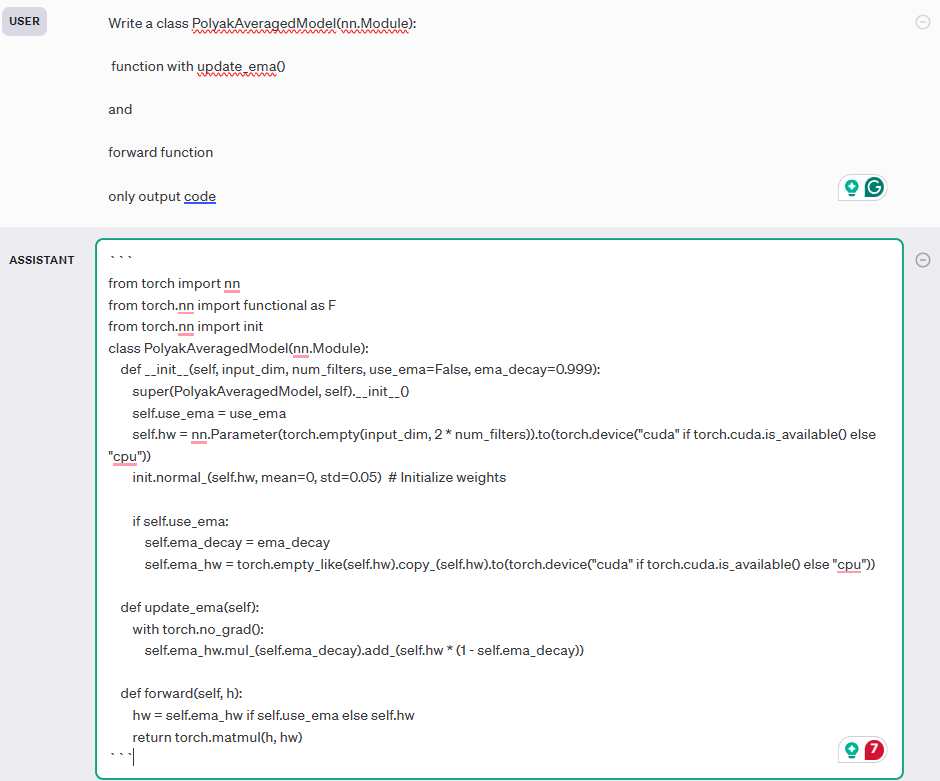
\includegraphics[width=0.5\textwidth]{report_data/g-1.png}
    \caption{GPT chat history}
\end{figure}


\begin{figure}
    \centering
    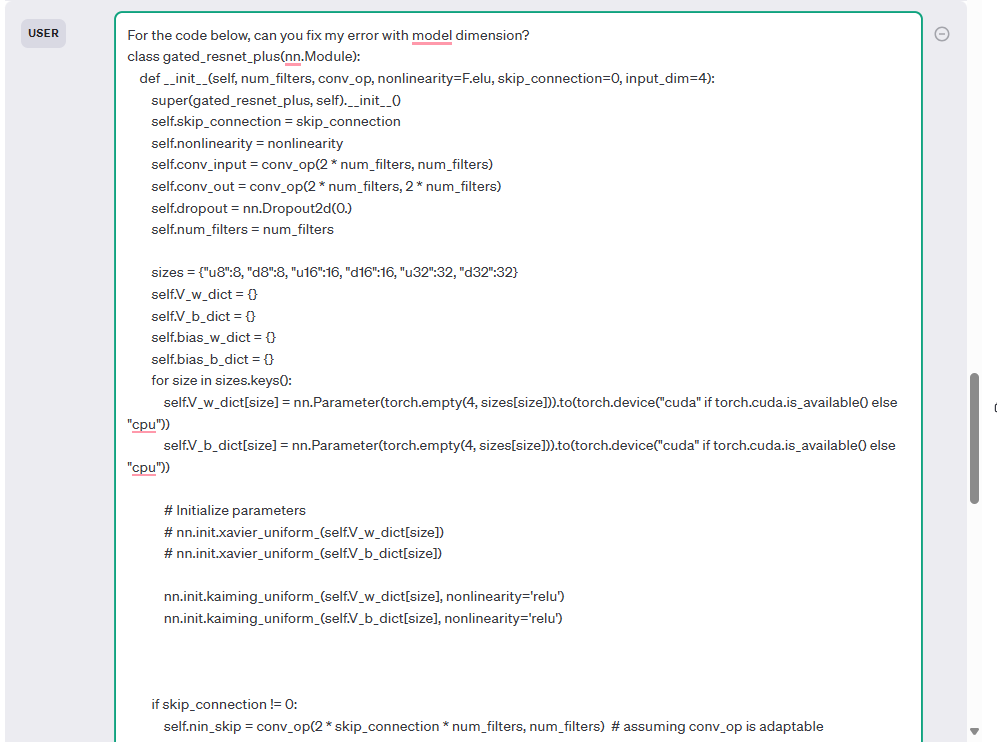
\includegraphics[width=0.5\textwidth]{report_data/g-2.png}
    \caption{GPT chat history}
\end{figure}


\begin{figure}
    \centering
    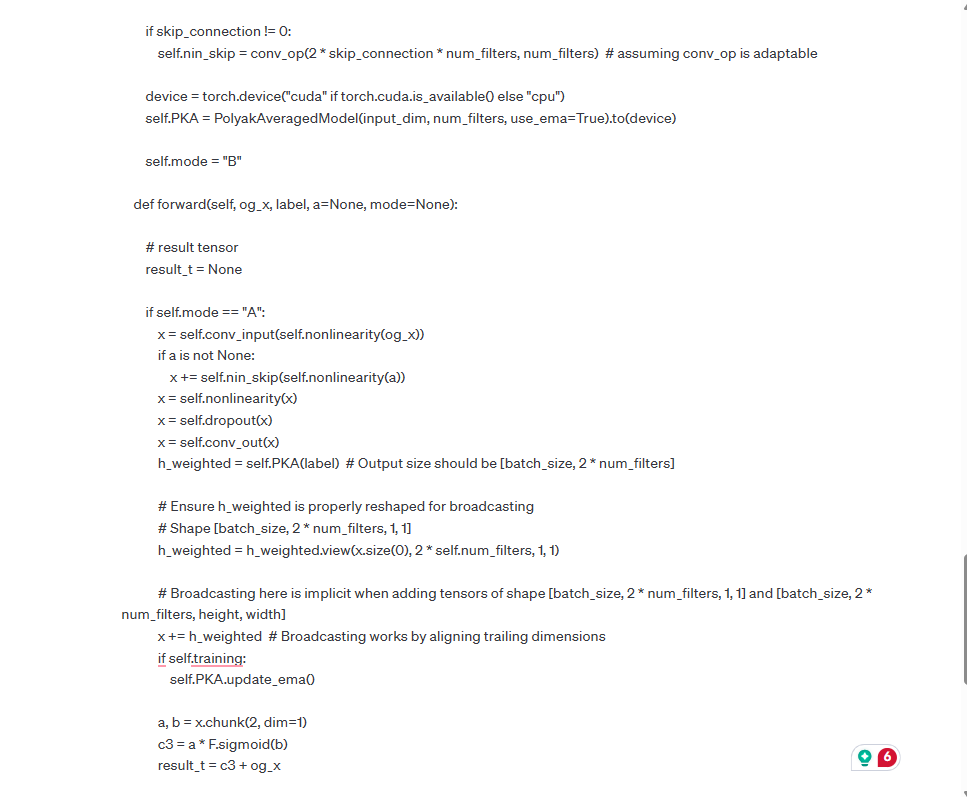
\includegraphics[width=0.5\textwidth]{report_data/g-3.png}
    \caption{GPT chat history}
\end{figure}


\begin{figure}
    \centering
    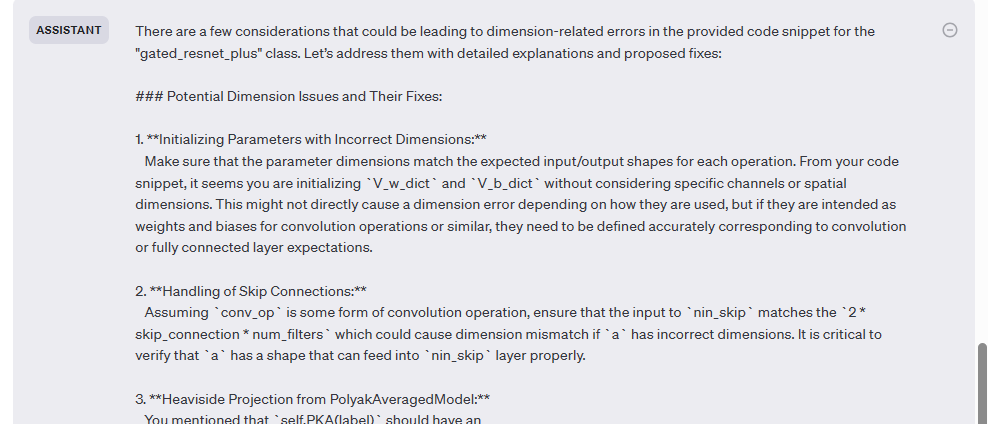
\includegraphics[width=0.5\textwidth]{report_data/g-4.png}
    \caption{GPT chat history}
\end{figure}


\begin{figure}
    \centering
    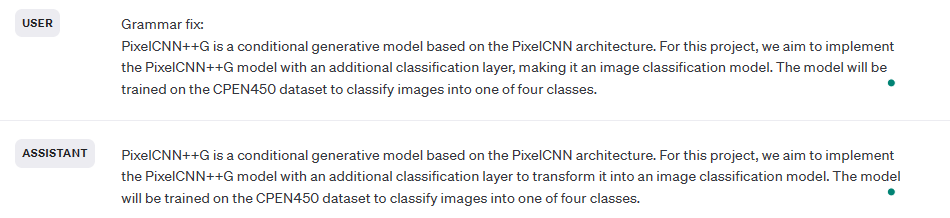
\includegraphics[width=0.5\textwidth]{report_data/g-5.png}
    \caption{GPT chat history}
\end{figure}


\begin{figure}
    \centering
    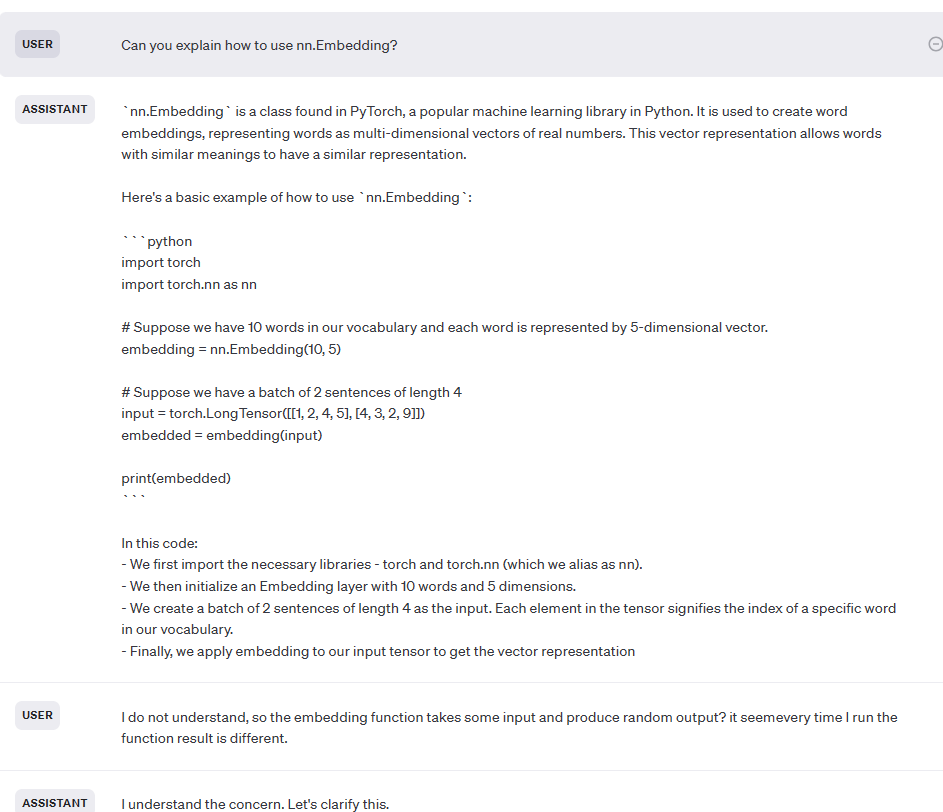
\includegraphics[width=0.5\textwidth]{report_data/g-6.png}
    \caption{GPT chat history}
\end{figure}


\begin{figure}
    \centering
    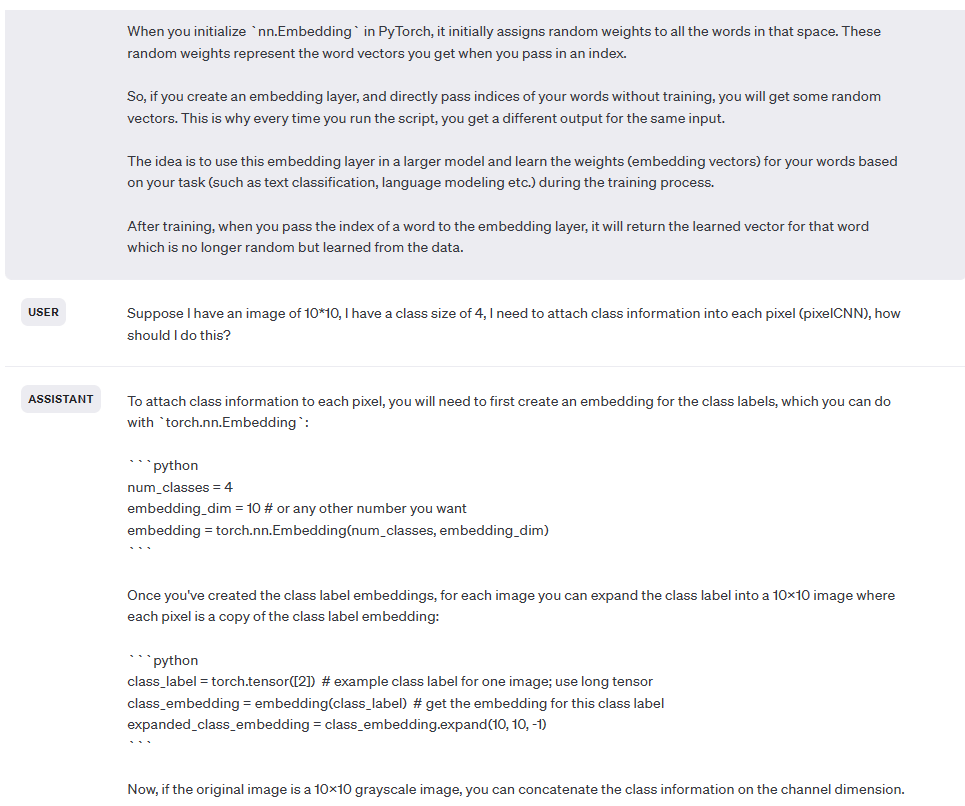
\includegraphics[width=0.5\textwidth]{report_data/g-7.png}
    \caption{GPT chat history}
\end{figure}


\begin{figure}
    \centering
    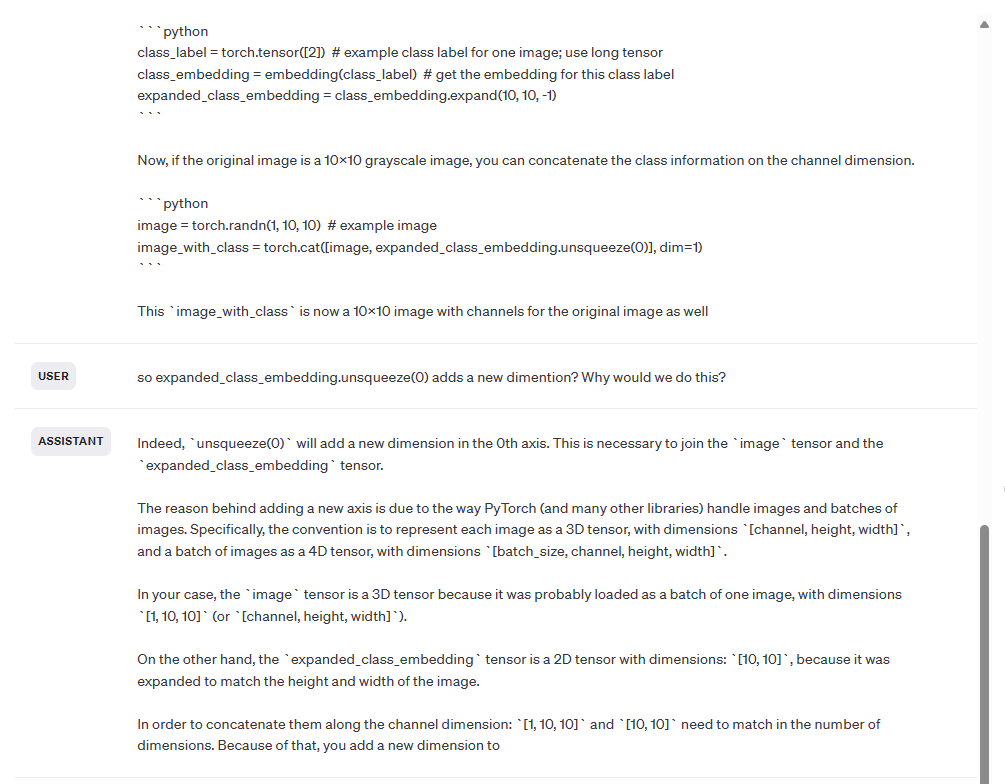
\includegraphics[width=0.5\textwidth]{report_data/g-8.png}
    \caption{GPT chat history}
\end{figure}


\begin{figure}
    \centering
    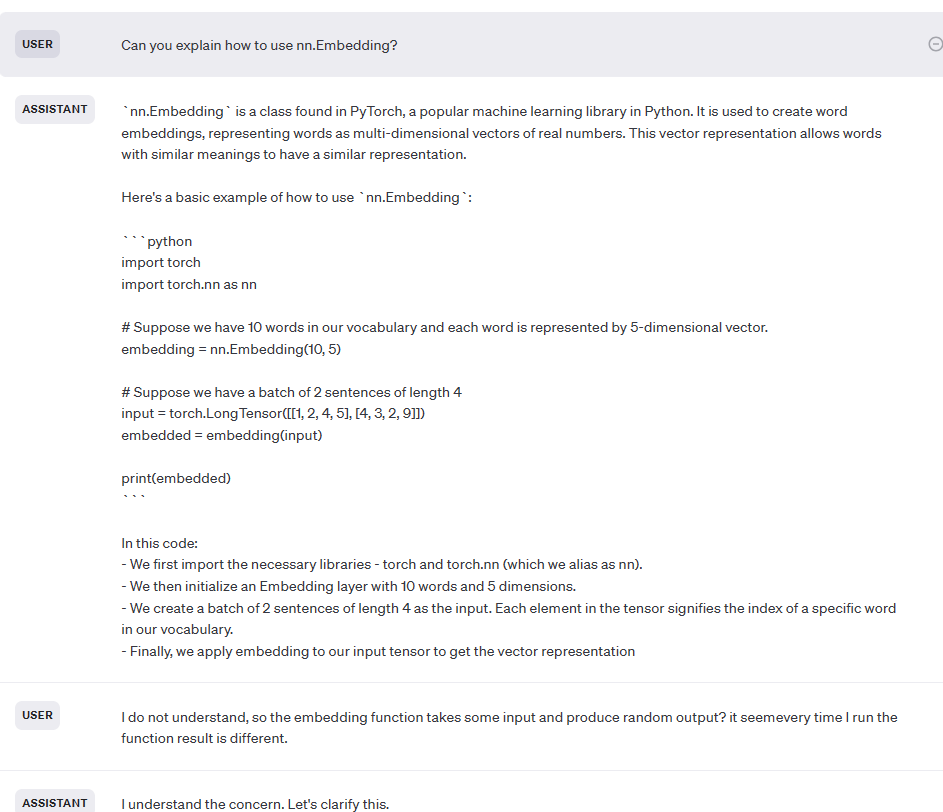
\includegraphics[width=0.5\textwidth]{report_data/g-9.png}
    \caption{GPT chat history}
\end{figure}


\begin{figure}
    \centering
    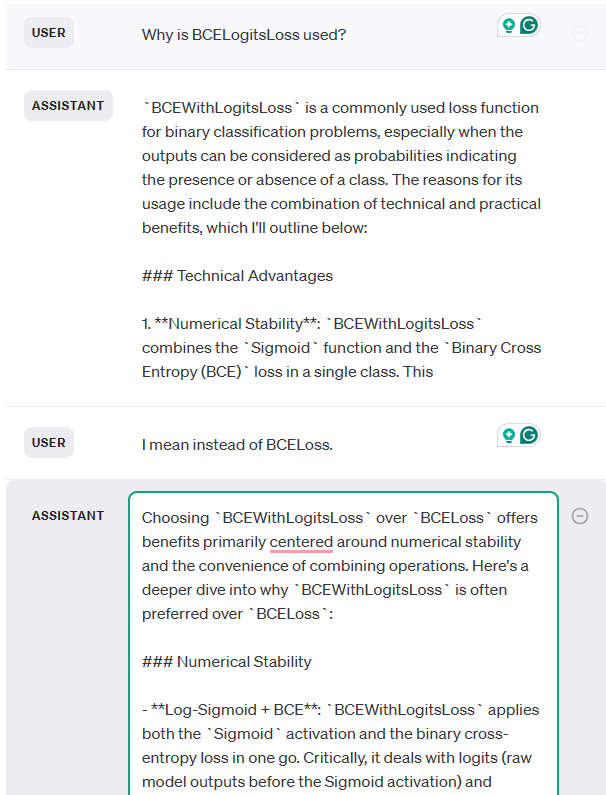
\includegraphics[width=0.5\textwidth]{report_data/g-10.png}
    \caption{GPT chat history}
\end{figure}


\begin{figure}
    \centering
    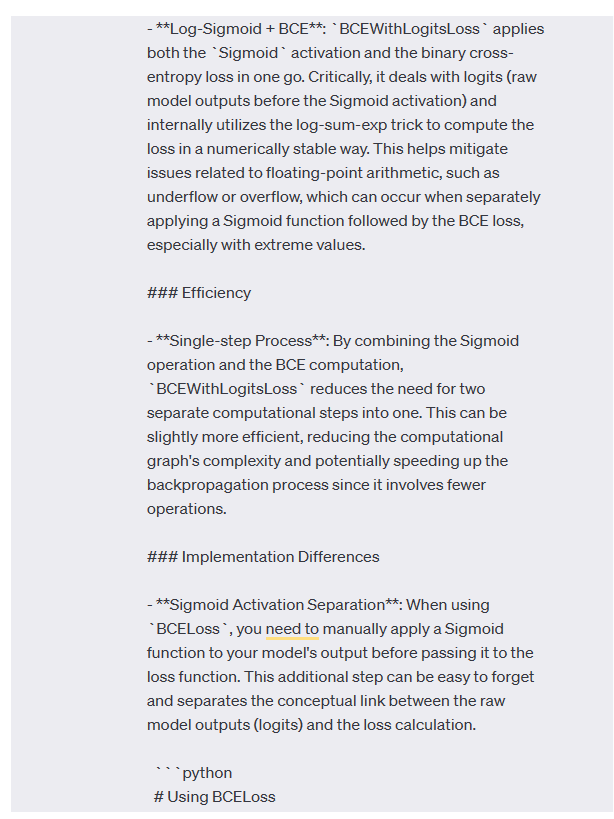
\includegraphics[width=0.5\textwidth]{report_data/g-11.png}
    \caption{GPT chat history}
\end{figure}


\begin{figure}[H]
    \centering
    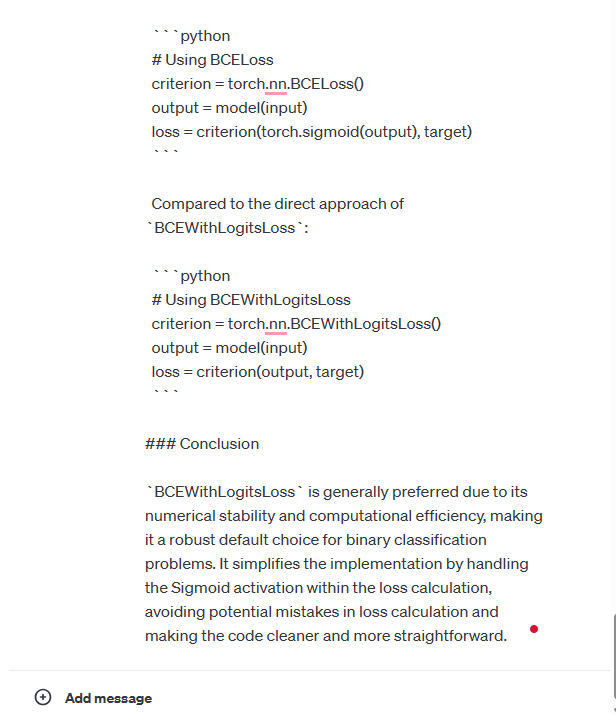
\includegraphics[width=0.5\textwidth]{report_data/g-12.png}
    \caption{GPT chat history}
\end{figure}

\section*{References}
[1] T. van den Salimans, A. Karpathy, X. Chen, and D. p. Kingma, PIXELCNN++: IMPROVING THE PIXELCNN WITH DISCRETIZED LOGISTIC MIXTURE LIKELIHOOD AND OTHER MODIFICATIONS, 2017. Accessed: 2024. [Online]. Available: https://arxiv.org/pdf/1606.05328.pdf
[2] A. van den Oord et al., Conditional Image Generation with PixelCNN Decoders, 2016. Accessed: 2024. [Online]. Available: https://arxiv.org/pdf/1606.05328.pdf

\end{document}